\documentclass[aspectratio=169,11pt]{ctexbeamer}

\usepackage{graphicx}
\usepackage{booktabs}
\usepackage{array}
\usepackage{amsmath}
\usepackage{xcolor}
\usepackage{tikz}
\usepackage{fontawesome5}

\usetheme{default}
\setbeamertemplate{navigation symbols}{}
\setbeamertemplate{footline}{}

\definecolor{Ink}{HTML}{102A43}
\definecolor{Teal}{HTML}{0F766E}
\definecolor{Orange}{HTML}{E8783C}
\definecolor{Paper}{HTML}{F7F6F2}
\definecolor{Mist}{HTML}{DDECE9}
\definecolor{SoftBlue}{HTML}{E7EEF6}
\definecolor{Gray}{HTML}{52616B}

\setbeamercolor{normal text}{fg=Ink,bg=Paper}
\setbeamercolor{frametitle}{fg=Ink,bg=Paper}
\setbeamercolor{structure}{fg=Teal}
\setbeamercolor{alerted text}{fg=Orange}
\setbeamerfont{frametitle}{size=\Large,series=\bfseries}
\setbeamerfont{normal text}{size=\large}
\setbeamerfont{title}{size=\fontsize{25}{30}\selectfont,series=\bfseries}
\setbeamerfont{subtitle}{size=\large}
\setbeamersize{text margin left=0.65cm,text margin right=0.65cm}

\newcommand{\tealbold}[1]{\textcolor{Teal}{\textbf{#1}}}
\newcommand{\warn}[1]{\textcolor{Orange}{\textbf{#1}}}
\newcommand{\pill}[1]{\tikz[baseline=(X.base)]\node[fill=Mist,rounded corners=2pt,inner xsep=6pt,inner ysep=3pt] (X) {\small\textbf{#1}};}
\newcommand{\source}[1]{%
  \vfill
  \begin{tikzpicture}[remember picture,overlay]
    \fill[Ink] (current page.south west) rectangle ([yshift=0.35cm]current page.south east);
    \node[anchor=west,text=white,font=\fontsize{4.8}{5.6}\selectfont,align=left,text width=14.25cm]
      at ([xshift=0.28cm,yshift=0.17cm]current page.south west) {#1};
    \node[anchor=east,text=white,font=\scriptsize]
      at ([xshift=-0.20cm,yshift=0.17cm]current page.south east) {\insertframenumber};
  \end{tikzpicture}%
}

\setbeamertemplate{frametitle}{%
  \vspace{0.20cm}\insertframetitle\par
  \vspace{-0.08cm}\textcolor{Teal}{\rule{1.0cm}{1.3pt}}\vspace{0.12cm}
}

\title{3D-VLA 入门导读}
\subtitle{机器人如何“看懂三维世界、想象目标状态、再规划动作”}
\author{第一次组会}
\date{\today}

\begin{document}

% 1
\begin{frame}[plain]
  \begin{columns}[T,onlytextwidth]
    \begin{column}{0.53\textwidth}
      \vspace{0.65cm}
      {\usebeamerfont{title}\color{Ink}\inserttitle\par}
      \vspace{0.28cm}
      {\usebeamerfont{subtitle}\color{Gray}\insertsubtitle\par}
      \vspace{0.48cm}
      \pill{3D perception}\quad\pill{world model}\quad\pill{robot action}
      \vspace{0.72cm}

      {\large 面向没有 VLA 背景的组员}\par
      \vspace{0.08cm}
      {\small 目标：听完能讲清楚问题、方法和证据边界}
    \end{column}
    \begin{column}{0.44\textwidth}
      \vspace{0.52cm}
      \includegraphics[page=3,trim=28 480 28 24,clip,width=\linewidth]{../references/zhen24a-3d-vla.pdf}
      \vspace{0.15cm}
      {\scriptsize\color{Gray}图：3D-VLA 的“目标想象—动作生成”管线}
    \end{column}
  \end{columns}
  \source{Ref.: [1] H. Zhen \emph{et al.}, ``3D-VLA: A 3D Vision-Language-Action Generative World Model,'' in \emph{Proc. ICML}, vol. 235, 2024, pp. 60258--60276.}
\end{frame}

% 2
\begin{frame}{先理解 VLA：把机器人控制写成“下一段 token”}
  \vspace{0.15cm}
  \begin{columns}[c,onlytextwidth]
    \begin{column}{0.58\textwidth}
      {\fontsize{17}{22}\selectfont\centering
        \textbf{视觉观测 $I_t$ + 语言指令 $x$}\par
        \vspace{0.12cm}$\Downarrow$\par\vspace{0.12cm}
        \textbf{动作 token 序列 $a_{t:t+H}$}\par
      }
      \vspace{0.15cm}
      \begin{itemize}
        \item \textbf{Vision}：相机看到什么
        \item \textbf{Language}：人希望机器人做什么
        \item \textbf{Action}：机械臂位置、旋转与夹爪开合
      \end{itemize}
    \end{column}
    \begin{column}{0.38\textwidth}
      \begin{beamercolorbox}[sep=0.40cm,rounded=true]{block body}
        \small\textbf{RT-2 的关键做法}\par\vspace{0.18cm}
        把机器人动作离散成文本 token，让视觉语言模型同时学习网页知识与机器人轨迹。
      \end{beamercolorbox}
      \vspace{0.34cm}
      \alert{但普通 VLA 多数依赖 2D 图像，并直接从观测预测动作。}
    \end{column}
  \end{columns}
  \source{Refs.: [1] A. Brohan \emph{et al.}, ``RT-2: Vision-Language-Action Models Transfer Web Knowledge to Robotic Control,'' in \emph{Proc. CoRL}, 2023, pp. 2165--2183. [2] H. Zhen \emph{et al.}, \emph{Proc. ICML}, 2024.}
\end{frame}

% 3
\begin{frame}{3D-VLA 针对两个缺口}
  \vspace{0.12cm}
  \renewcommand{\arraystretch}{1.42}
  \begin{tabular}{>{\bfseries}p{0.18\textwidth} p{0.36\textwidth} p{0.37\textwidth}}
    \toprule
    & 常见 2D VLA & 3D-VLA 的选择 \\
    \midrule
    空间理解 & 图像像素提供间接线索 & RGB-D、点云和 3D 包围盒明确表达距离与位置 \\
    动作生成 & 观测直接映射到动作 & 先生成目标图像或目标点云，再据此预测动作 \\
    世界动态 & 隐含在策略参数中 & 用生成模型显式“想象”任务完成后的状态 \\
    输出形式 & 语言或动作 & 语言、位置、图像、深度、点云与动作 token \\
    \bottomrule
  \end{tabular}
  \vspace{0.38cm}

  \centering
  {\large\tealbold{核心假设：目标状态是连接语言意图与机器人动作的中间表示。}}
  \source{Ref.: [1] H. Zhen \emph{et al.}, ``3D-VLA: A 3D Vision-Language-Action Generative World Model,'' in \emph{Proc. ICML}, vol. 235, 2024, pp. 60258--60276.}
\end{frame}

% 4
\begin{frame}{总体架构：理解场景、想象目标、生成动作}
  \centering
  \includegraphics[page=3,trim=24 535 24 18,clip,width=0.80\linewidth]{../references/zhen24a-3d-vla.pdf}
  \vspace{0.12cm}

  \begin{columns}[T,onlytextwidth]
    \begin{column}{0.31\textwidth}
      \textbf{1. 场景编码}\par
      多视角图像形成 3D 特征，经 Q-Former 接入语言模型。
    \end{column}
    \begin{column}{0.31\textwidth}
      \textbf{2. 目标想象}\par
      LLM 的输出经 projector 条件化扩散模型，生成目标图像或点云。
    \end{column}
    \begin{column}{0.31\textwidth}
      \textbf{3. 机器人控制}\par
      目标状态再次送入模型，输出离散动作 token。
    \end{column}
  \end{columns}
  \source{Ref.: [1] H. Zhen \emph{et al.}, ``3D-VLA: A 3D Vision-Language-Action Generative World Model,'' in \emph{Proc. ICML}, vol. 235, 2024, Fig. 2.}
\end{frame}

% 5
\begin{frame}{一个模型覆盖三类任务}
  \centering
  \includegraphics[page=2,trim=23 470 23 26,clip,width=0.70\linewidth]{../references/zhen24a-3d-vla.pdf}
  \vspace{0.10cm}

  \begin{columns}[T,onlytextwidth]
    \begin{column}{0.32\textwidth}
      \tealbold{推理与定位}\par
    \end{column}
    \begin{column}{0.32\textwidth}
      \tealbold{多模态目标生成}\par
    \end{column}
    \begin{column}{0.32\textwidth}
      \tealbold{机器人规划}\par
    \end{column}
  \end{columns}
  \source{Ref.: [1] H. Zhen \emph{et al.}, ``3D-VLA: A 3D Vision-Language-Action Generative World Model,'' in \emph{Proc. ICML}, vol. 235, 2024, Fig. 1.}
\end{frame}

% 6
\begin{frame}{数据构建：从已有视频补出 3D 监督}
  \vspace{0.18cm}
  \begin{columns}[c,onlytextwidth]
    \begin{column}{0.60\textwidth}
      \begin{enumerate}
        \item 汇集机器人操作与人—物交互数据
        \item 用 ZoeDepth 补深度，用 RAFT 对齐视频帧
        \item 用 Grounded-SAM 提取目标物体掩码，再投影为点云与 3D 包围盒
        \item 用模板和语言模型生成问答、定位、目标生成与动作预测指令
      \end{enumerate}
    \end{column}
    \begin{column}{0.36\textwidth}
      \begin{beamercolorbox}[sep=0.42cm,rounded=true]{block body}
        {\fontsize{32}{36}\selectfont\color{Teal}\textbf{2M}}\par
        3D—语言—动作数据对
        \vspace{0.34cm}

        {\fontsize{27}{31}\selectfont\color{Orange}\textbf{316k}}\par
        使用的原始 episode
      \end{beamercolorbox}
      \vspace{0.20cm}
      {\scriptsize 论文汇总了 12 个 Open-X 子集，并加入 Dobb-E、RH20T、RLBench、CALVIN 与 HOI 数据。}
    \end{column}
  \end{columns}
  \source{Refs.: [1] H. Zhen \emph{et al.}, \emph{Proc. ICML}, 2024, Sec. 3 and Table 8. [2] A. Padalkar \emph{et al.}, ``Open X-Embodiment: Robotic Learning Datasets and RT-X Models,'' in \emph{Proc. ICRA}, 2024, pp. 6892--6903.}
\end{frame}

% 7
\begin{frame}{3D 表征提供“在哪里”和“有多远”}
  \begin{columns}[c,onlytextwidth]
    \begin{column}{0.52\textwidth}
      \includegraphics[page=17,trim=28 365 28 22,clip,width=\linewidth]{../references/zhen24a-3d-vla.pdf}
    \end{column}
    \begin{column}{0.44\textwidth}
      \textbf{点云}\par
      每个点带有 $(x,y,z)$ 坐标，可直接表达物体的三维形状和距离。
      \vspace{0.32cm}

      \textbf{3D 包围盒}\par
      用 6 个离散位置 token 表示轴对齐包围盒，帮助模型定位被操作物体。
      \vspace{0.32cm}

      \textbf{重要限制}\par
      真实相机的深度尺度和噪声并不统一，点云质量会影响控制精度。
    \end{column}
  \end{columns}
  \source{Ref.: [1] H. Zhen \emph{et al.}, ``3D-VLA: A 3D Vision-Language-Action Generative World Model,'' in \emph{Proc. ICML}, vol. 235, 2024, Secs. 3.2, 4.2.2, Fig. 6.}
\end{frame}

% 8
\begin{frame}[fragile]{交互 token：把物体、空间和动作塞进语言序列}
  \vspace{0.08cm}
  \begin{columns}[T,onlytextwidth]
    \begin{column}{0.43\textwidth}
      \textbf{场景与物体}
      \begin{itemize}
        \item \texttt{<scene> ... </scene>}
        \item \texttt{<obj> apple </obj>}
        \item \texttt{<loc0-255>} 表示 3D 坐标
      \end{itemize}
      \vspace{0.20cm}
      \textbf{动作}
      \begin{itemize}
        \item 位置 \texttt{<aloc0-255>}
        \item 旋转 \texttt{<arot0-255>}
        \item 夹爪 \texttt{<gripper0/1>}
      \end{itemize}
    \end{column}
    \begin{column}{0.53\textwidth}
      \begin{beamercolorbox}[sep=0.38cm,rounded=true]{block body}
        {\small\ttfamily
        User: Find some snacks for me.\\[0.18cm]
        Robot: I should \\
        <img> pick up <obj> chip bag </obj>\\
        <loc...> </img>}
      \end{beamercolorbox}
      \vspace{0.34cm}
      离散化让同一个语言模型接口同时处理语义、空间位置与机器人动作，但也会牺牲连续控制的精度。
    \end{column}
  \end{columns}
  \source{Ref.: [1] H. Zhen \emph{et al.}, ``3D-VLA: A 3D Vision-Language-Action Generative World Model,'' in \emph{Proc. ICML}, vol. 235, 2024, Sec. 4.2.2.}
\end{frame}

% 9
\begin{frame}{生成式世界模型：先画出任务完成后的样子}
  \centering
  \includegraphics[page=7,trim=22 420 22 22,clip,width=0.55\linewidth]{../references/zhen24a-3d-vla.pdf}
  \vspace{0.10cm}

  \begin{columns}[T,onlytextwidth]
    \begin{column}{0.47\textwidth}
      \textbf{RGB-D 目标生成}\par
      Stable Diffusion 1.4 接收初始 RGB-D 与指令，编辑出目标 RGB-D。
    \end{column}
    \begin{column}{0.47\textwidth}
      \textbf{点云目标生成}\par
      Point-E 接收初始点云与指令，生成任务完成后的点云。
    \end{column}
  \end{columns}
  \source{Refs.: [1] H. Zhen \emph{et al.}, \emph{Proc. ICML}, 2024, Sec. 4.3 and Fig. 3. [2] R. Rombach \emph{et al.}, ``High-Resolution Image Synthesis with Latent Diffusion Models,'' in \emph{Proc. CVPR}, 2022, pp. 10684--10695.}
\end{frame}

% 10
\begin{frame}{训练分成三步，最后只对齐必要参数}
  \vspace{0.18cm}
  \begin{columns}[T,onlytextwidth]
    \begin{column}{0.31\textwidth}
      {\color{Teal}\Large\textbf{01}}\par
      \textbf{适配扩散模型}\par\vspace{0.12cm}
      在机器人数据上训练 RGB-D 编辑与点云生成，缩小互联网图像与机器人场景的域差异。
    \end{column}
    \begin{column}{0.31\textwidth}
      {\color{Teal}\Large\textbf{02}}\par
      \textbf{训练多模态 LLM}\par\vspace{0.12cm}
      基于 BLIP-2 FlanT5-XL，训练问答、描述、定位与动作预测。
    \end{column}
    \begin{column}{0.31\textwidth}
      {\color{Teal}\Large\textbf{03}}\par
      \textbf{跨模态对齐}\par\vspace{0.12cm}
      联合优化特殊 token、projector 与扩散模型 LoRA，同时最小化语言损失和去噪损失。
    \end{column}
  \end{columns}
  \vspace{0.55cm}
  \begin{beamercolorbox}[sep=0.32cm,rounded=true]{block body}
    \centering\textbf{工程代价不小：论文各阶段使用了数百张 V100 GPU。}
  \end{beamercolorbox}
  \source{Refs.: [1] H. Zhen \emph{et al.}, \emph{Proc. ICML}, 2024, Appendix A. [2] E. J. Hu \emph{et al.}, ``LoRA: Low-Rank Adaptation of Large Language Models,'' in \emph{Proc. ICLR}, 2022.}
\end{frame}

% 11
\begin{frame}{证据一：3D 数据显著改善推理与定位}
  \begin{columns}[c,onlytextwidth]
    \begin{column}{0.53\textwidth}
      \textbf{语言任务代表结果}\par\vspace{0.12cm}
      \renewcommand{\arraystretch}{1.25}
      \resizebox{\linewidth}{!}{\begin{tabular}{lrr}
        \toprule
        任务与指标 & BLIP-2 & \textbf{3D-VLA} \\
        \midrule
        Embodied QA, BLEU-4 & 15.48 & \textbf{26.80} \\
        Task caption, BLEU-4 & 3.16 & \textbf{34.88} \\
        What-if QA, BLEU-4 & 0.06 & \textbf{29.38} \\
        Dense caption, EM@1 & 13.10 & \textbf{39.49} \\
        \bottomrule
      \end{tabular}}
    \end{column}
    \begin{column}{0.43\textwidth}
      \textbf{3D 定位结果}\par\vspace{0.12cm}
      \renewcommand{\arraystretch}{1.25}
      \resizebox{\linewidth}{!}{\begin{tabular}{lrr}
        \toprule
        方法 & IoU & Acc@25 \\
        \midrule
        Kosmos-2 + GT depth & 10.92 & 12.73 \\
        CoVLM + GT depth & 19.81 & 25.39 \\
        \textbf{3D-VLA} & \textbf{29.33} & \textbf{42.26} \\
        \bottomrule
      \end{tabular}}
      \vspace{0.28cm}

      {\small\warn{解读边界：}这些任务主要使用 held-in 数据，说明 3D 监督有效，不等同于开放世界泛化。}
    \end{column}
  \end{columns}
  \source{Ref.: [1] H. Zhen \emph{et al.}, ``3D-VLA: A 3D Vision-Language-Action Generative World Model,'' in \emph{Proc. ICML}, vol. 235, 2024, Tables 1--2.}
\end{frame}

% 12
\begin{frame}{证据二：目标想象帮助部分机器人任务}
  \begin{columns}[T,onlytextwidth]
    \begin{column}{0.51\textwidth}
      \textbf{RLBench 成功率（\%）}\par\vspace{0.10cm}
      \renewcommand{\arraystretch}{1.22}
      \resizebox{\linewidth}{!}{\begin{tabular}{lrrrr}
        \toprule
        方法 & 放刀 & 取伞 & 拿杯 & 未见杯 \\
        \midrule
        无目标生成 & 58 & 68 & 34 & 24 \\
        \textbf{3D-VLA} & \textbf{68} & \textbf{80} & \textbf{40} & \textbf{28} \\
        \bottomrule
      \end{tabular}}
      \vspace{0.30cm}
      目标状态对需要定位与辨别目标的任务帮助更明显。
    \end{column}
    \begin{column}{0.45\textwidth}
      \textbf{CALVIN 长序列任务}\par\vspace{0.10cm}
      \renewcommand{\arraystretch}{1.22}
      \resizebox{\linewidth}{!}{\begin{tabular}{lrrr}
        \toprule
        方法 & 完成 1 个 & 完成 3 个 & 平均长度 \\
        \midrule
        MCIL & 28.2 & 0.3 & 0.31 \\
        \textbf{3D-VLA} & \textbf{44.7} & \textbf{8.1} & \textbf{0.71} \\
        \bottomrule
      \end{tabular}}
      \vspace{0.30cm}
      {\small\warn{仍有限：}连续完成 5 个任务的成功率为 0，RLBench 使用开环执行。}
    \end{column}
  \end{columns}
  \vspace{0.28cm}
  {\small 图像目标生成中，3D-VLA 取得 PSNR 17.21、SSIM 0.636；FID 并非所有方法中最低，因此应分指标阅读。}
  \source{Refs.: [1] H. Zhen \emph{et al.}, \emph{Proc. ICML}, 2024, Tables 3, 5--6. [2] S. James \emph{et al.}, ``RLBench: The Robot Learning Benchmark and Learning Environment,'' \emph{IEEE RA-L}, vol. 5, no. 2, pp. 3019--3026, 2020.}
\end{frame}

% 13
\begin{frame}{论文明确承认的四类局限}
  \vspace{0.16cm}
  \begin{columns}[T,onlytextwidth]
    \begin{column}{0.48\textwidth}
      \textbf{精细控制不足}\par
      3D 特征与离散动作 token 难以支持小物体的精确抓取。
      \vspace{0.30cm}

      \textbf{目标图像会“幻觉”}\par
      纹理或形状变化、物体消失、生成错误任务结果或完全不变化。
    \end{column}
    \begin{column}{0.48\textwidth}
      \textbf{真实深度噪声}\par
      不同场景尺度不一致，深度图与点云质量下降。
      \vspace{0.30cm}

      \textbf{数据质量长尾}\par
      不同数据集的标注和图像质量差异明显，表现随数据源波动。
    \end{column}
  \end{columns}
  \vspace{0.50cm}
  \begin{beamercolorbox}[sep=0.34cm,rounded=true]{block body}
    \centering\textbf{讨论时要区分：生成了“合理目标图”与机器人真正闭环完成任务。}
  \end{beamercolorbox}
  \source{Ref.: [1] H. Zhen \emph{et al.}, ``3D-VLA: A 3D Vision-Language-Action Generative World Model,'' in \emph{Proc. ICML}, vol. 235, 2024, Sec. 6.}
\end{frame}

% 14
\begin{frame}{带走的三个认识与讨论问题}
  \begin{columns}[T,onlytextwidth]
    \begin{column}{0.55\textwidth}
      \textbf{三个认识}
      \begin{enumerate}
        \item 3D 表征把空间关系从隐式线索变成显式监督。
        \item 目标状态生成给动作预测增加了可解释的中间变量。
        \item 论文证明了方法潜力，但真实闭环控制和跨场景泛化仍未充分验证。
      \end{enumerate}
    \end{column}
    \begin{column}{0.41\textwidth}
      \textbf{建议讨论}
      \begin{itemize}
        \item 目标图像和目标点云，哪个更适合控制？
        \item 离散动作 token 如何兼顾语义与精度？
        \item 如果复现，最小可行实验应选哪一部分？
      \end{itemize}
      \vspace{0.28cm}
      \begin{beamercolorbox}[sep=0.30cm,rounded=true]{block body}
        \centering 下一步：先跑目标图像生成 demo，再设计小规模消融实验。
      \end{beamercolorbox}
    \end{column}
  \end{columns}
  \source{Ref.: [1] H. Zhen \emph{et al.}, ``3D-VLA: A 3D Vision-Language-Action Generative World Model,'' in \emph{Proc. ICML}, vol. 235, 2024, pp. 60258--60276.}
\end{frame}

\end{document}
